\documentclass[8pt]{beamer}

\setbeamertemplate{background canvas}[vertical shading][bottom=cyan!10,top=blue!10]

\usetheme{Warsaw}
\usefonttheme[onlysmall]{structurebold}

% pour le fichiers .pdf
\usepackage{graphicx}
\usepackage{color}
% pour les fichiers .png
% \usepackage{pgf,pgfarrows}
% \usepackage{pgf,pgfarrows}
\usepackage{amsmath,amssymb}
\usepackage[latin1]{inputenc}
\usepackage[T1]{fontenc}
%\usepackage[french]{babel}
\usepackage{textcomp}
\usepackage{multitoc}
\usepackage{mdwtab}
\setbeamercovered{dynamic}
\DeclareMathOperator*{\argmin}{argmin}

\title[Compilation infrastructure (1/2)]{Compilation infrastructure (1/2)}
\author[OpenTURNS Consortium, 2019]
{
  Trainer : R�gis LEBRUN, EADS/IW/SE/AM
  regis.lebrun@eads.net
}



\date[March 22-25th 2011]
{
  Developers training \\

  \begin{center}
    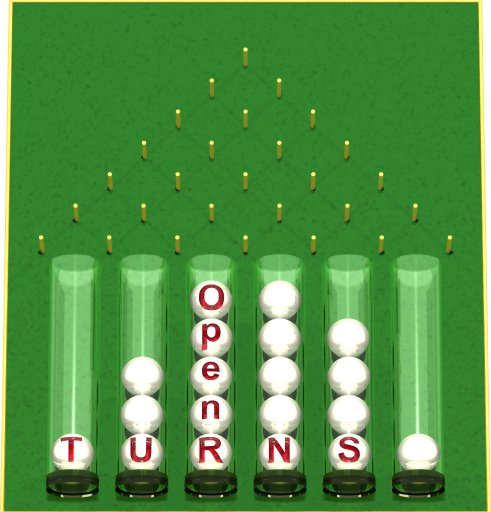
\includegraphics[height=2cm]{logoOT.jpg}
  \end{center}
}

\subject{OpenTURNS Developers Training}

% \part<presentation>{Corps de presentation}


\begin{document}

\frame{\titlepage}

% necessaire pour la table des matieres
\part{Main part}

% table des matieres
\begin{frame}
  \frametitle{OpenTURNS compilation infrastructure}
  \tableofcontents[part=1]
\end{frame}
%%%%%%%%%%%%%%%%%%%%%%%%% 
% The OpenTURNS package %
%%%%%%%%%%%%%%%%%%%%%%%%% 
\section[Autotools, CMake]{Autotools, CMake}
%%%%%%%%%%%%% 
% The tools %
%%%%%%%%%%%%% 
\begin{frame}
  \frametitle{Two compilation infrastructures}
  \begin{block}{The autotools}
    The autotools are a set of tools that aim to ease the configuration and compilation of large software projects in the UNIX world. The objective is to generate Makefiles from a set of templates and the information gathered during a configuration step. The main tools are:
    \begin{itemize}
    \item \emph{aclocal} in charge of the management of the several \emph{detection macros} needed for the configuration of the project: the dependencies, the compilers and so on.
    \item \emph{automake} in charge of producing parameterized Makefiles (\emph{Makefile.in}) from template Makefiles (\emph{Makefiles.am}).
    \item \emph{autoconf} in charge of the parameterization of both the Makefiles and the sources of the project (notably for the conditional compilation of parts of the project). The main purpose of this tool is to produce a shell script (\emph{configure}) based on a template (\emph{autoconf.ac}) and the macros gathered by aclocal (\emph{aclocal.m4}). This shell script converts the parameterized Makefiles (Makefile.in) into ready to use Makefiles.
    \item \emph{autotest} in charge of the unit tests. Such a test is described as an association between a shell script command to be executed and a reference standard output and error output that is expected. The validation is done using a character-based comparison of the shell script output and the reference output, and through the return code of the shell script command.
    \end{itemize}
  \end{block}
\end{frame}

\begin{frame}
  \frametitle{Two compilation infrastructures}
  \begin{block}{CMake}
    CMake is another compilation infrastructure with the same objectives as the autotools. All the configuration is done through a hierarchy of text files written in the CMake macro language, and a GUI is available to ease the creation of this hierarchy. The same topics are covered:
    \begin{itemize}
    \item \emph{dependency detection} through a set of detection macros: the several .cmake files;
    \item \emph{configuration} through a master configuration file: the top-level CMakeLists.txt file;
    \item \emph{source organization} through a set of CMakeLists.txt files disseminated in the whole source tree: each such file includes the declaration of the several source files and associated header files, and make a recursive call to the subdirectories.
    \item \emph{testing} using a mechanism that is not completely clear to me at this time...
    \end{itemize}
  \end{block}
\end{frame}
%%%%%%%%%%%%%%%%%% 
% Development process
%%%%%%%%%%%%%%%%%% 
\section[Development process]{Development process}
\begin{frame}
  \frametitle{Development process}
  \begin{block}{Two main situations}
    There are two distinct situations in the development of additional capabilities of OpenTURNS:
    \begin{itemize}
      \item The addition of a new instance of an existing concept;
      \item The introduction of a new concept.
    \end{itemize}
    The associated development process shares the same principles in both cases, but the details are more involved in the second case.\\
    Both cases are covered in the \alert{Contribution Guide} documentation that comes with OpenTURNS, only the first situation will be covered here. We suppose that our extension consist in the creation of a new class called MyClass in an existing directory.
  \end{block}
\end{frame}
%%%%%%%%%%%%%%%%%%% 
% Add a new class
%%%%%%%%%%%%%%%%%%% 
\begin{frame}
  \frametitle{Populate an existing concept}
  \begin{block}{Step 1: create the header file and the associated source file}
    Create MyClass.hxx and MyClass.cxx in the same directory. The files must have the standard OpenTURNS header, with a brief description of the class using the Doxygen format and the standard reference to the LGPL license.
  
  For the header file MyClass.hxx, the interface must be embraced between the preprocessing clauses:
  
\begin{tabular}{l}
\ttfamily \#ifndef OPENTURNS\_MYCLASS\_HXX\\
\ttfamily \#define OPENTURNS\_MYCLASS\_HXX\\
\ttfamily ...\\
\ttfamily your interface\\
\ttfamily ...\\
\ttfamily \#endif OPENTURNS\_MYCLASS\_HXX
\end{tabular}
  
  to prevent from multiple inclusions.
  
  See any pair of .hxx/.cxx files in the current directory and the OpenTURNS Coding Rules document as a guide for your development: the use of namespaces, case convention for the static methods, the other methods and the attributes, the trailing underscore for the attribute names to name a few rules.
  \end{block}
\end{frame}
%%%%%%%%%%%%%%%%%% 
% Add a new class
%%%%%%%%%%%%%%%%%% 
\begin{frame}
  \frametitle{Populate an existing concept}
  \begin{block}{Step 2: update the automake file and the CMake file}
    Modify the Makefile.am file in the directory containing MyClass.hxx and MyClass.cxx:
    \begin{itemize}
    \item add MyClass.hxx to the {\ttfamily otinclude\_HEADERS} variable
    \item add MyClass.cxx to the {\ttfamily libOTXXXXXX\_la\_\_SOURCES} variable, where XXXXXX is the name of the current directory.
    \end{itemize}
    Modify the CMakeList.txt file in the same directory:
    \begin{itemize}
    \item add MyClass.hxx using the instruction {\ttfamily ot\_install\_header\_file ( MyClass.hxx )}
    \item add MyClass.cxx using the instruction {\ttfamily ot\_add\_source\_file ( MyClass.cxx )}
    \end{itemize}
  \end{block}
\end{frame}
%%%%%%%%%%%%%%%%%%
% Add a new class
%%%%%%%%%%%%%%%%%% 
\begin{frame}
  \frametitle{Populate an existing concept}
  \begin{block}{Step 3: the source code of the test(s)}
    Create a test file t\_MyClass\_std.cxx in the directory lib/test. This test file must check at least the standard functionalities of the class MyClass. If relevant, some specific aspects of the class can be checked in specific other test files, such as the exceptional behaviour of the class or its functionalities in extrem configurations (large data set, hard to solve problems etc.).
  \end{block}
\end{frame}
%%%%%%%%%%%%%%%%%%
% Add a new class
%%%%%%%%%%%%%%%%%% 
\begin{frame}
  \frametitle{Populate an existing concept}
  \begin{block}{Step 4: the autotest file(s) of the test(s)}
    Create an autotest file t\_MyClass\_std.at in the directory lib/test. This file describes the test, how to run it and what is the expected output (copy-paste the \emph{validated} output of the test in the proper section of t\_MyClass\_std.at).\\
    For the CMake infrastructure, there is no such step.
  \end{block}
\end{frame}
%%%%%%%%%%%%%%%%%%
% Add a new class
%%%%%%%%%%%%%%%%%% 
\begin{frame}
  \frametitle{Populate an existing concept}
  \begin{block}{Step 5: update the automake file and the CMake file of the lib/test directory}
  \begin{itemize}
  \item add t\_MyClass\_std (which is the name of the test executable) to the variable CHECK\_PROGS or INSTALLCHECK\_PROGS depending on the fact the test checks the correct behaviour of OpenTURNS independently of its installation or not. The several executables are organized following the library organization, you must follow this rule.
  \item add t\_MyClass\_std.at to the variable CHECK\_TESTS or INSTALLCHECK\_TESTS and in the correct set of autotest files, following the same rules than for the executable.
  \item Create a variable called t\_MyClass\_std\_SOURCES and set its value to t\_MyClass.cxx in the relevant set of sources.
  \end{itemize}
  For the CMake infrastructure, add the line ot\_installcheck\_test ( MyClass\_std ) in the relevant section of the CMakeLists.txt file.
  \end{block}
\end{frame}
%%%%%%%%%%%%%%%%%%
% Add a new class
%%%%%%%%%%%%%%%%%% 
\begin{frame}
  \frametitle{Populate an existing concept}
  \begin{block}{Step 6: update the autotest infrastructure}
    Add t\_MyClass\_std.at to the file check\_testsuite.at or installcheck\_testsuite.at using the same rule than for the Makefile.am modification.\\
    If the test checks functionalities available after the installation of OpenTURNS, use the installcheck\_testsuite.at file as your test is a post-installation test, else use the check\_testsuite.at file.\\
    There is no such step in the CMake infrastructure.
  \end{block}
\end{frame}
%%%%%%%%%%%%%%%%%%
% Add a new class
%%%%%%%%%%%%%%%%%% 
\begin{frame}
  \frametitle{Populate an existing concept}
  \begin{block}{Step 7: validation}
    If the validation of your class involved advanced mathematics, or was a significant work using other tools, you can add this validation in the validation/src directory.
    \begin{itemize}
    \item copy all of your files in the validation/src directory.
    \item modify the Makefile.am file by appending the list of your files to the dist\_validation\_DATA variable.
    \end{itemize}
  \end{block}
\end{frame}
%%%%%%%%%%%%%%%%%%
% Add a new class
%%%%%%%%%%%%%%%%%% 
\begin{frame}
  \frametitle{Document the new class}
  \begin{block}{Step 8: update the documentation}
    The documentation must be written in English, using LaTeX. For an addition to the C++ library, you may have to update the following documents in the OpenTURNS documentation source tree:
    \begin{itemize}
    \item Add an entry in the document src/ArchitectureGuide/OpenTURNS\_ArchitectureGuide.tex if your class has a significant impact on the library architecture.
    \item Add an entry in the document src/WrappersGuide/OpenTURNS\_WrappersGuide.tex if your class has a significant impact on the way OpenTURNS interfaces external codes.
    \item Add an entry in the document src/ReferenceGuide/OpenTURNS\_ReferenceGuide.tex if your class add a new concept not already described in the reference guide. Your entry must take the form of a specific description using the same template than the other descriptions.
    \end{itemize}
  \end{block}
\end{frame}
%%%%%%%%%%%%%%%%%%
% Critical points
%%%%%%%%%%%%%%%%%% 
\begin{frame}
  \frametitle{Tips and tricks}
  \begin{block}{Critical points}
    \begin{itemize}
    \item All the classes must include the {\ttfamily CLASSNAME} macro (defined in Base/Common/Object.hxx) in their header file in order to benefit from the (basic) introspection mechanisms. The associated {\ttfamily CLASSNAMEINIT} macro must be used in the corresponding source file.
    \item All the class corresponding to persistent objects must instantiate a static parameterized factory in their source file.
      \item In order to improve the readibility of the source code, the needed classes that are not in the current namespace must be aliased using a typedef. These typedef must be wisely separated between those in the header file and those in the source file.
      \item The const correctness of the code is very important, both for the signature of the methods and for the temporary variables.
      \item All the object arguments must be passed using const references. The use of non const references to make side effects must be limited as much as possible.
      \item Most of the coding rules are described in the Coding Rules Guide, but you can infer the rules by looking at the existing code. \alert{The key point is that the only difficult points should be the conception and the algorithms, not the indentation or the coding style!}
    \end{itemize}
  \end{block}
\end{frame}
%%%%%%%%%%%%%%%%%%
% Critical points
%%%%%%%%%%%%%%%%%% 
\begin{frame}
  \frametitle{Development of a new distribution}
  \begin{block}{Practical case: adding a new distribution to the C++ library}
    \begin{itemize}
    \item Each trainee has to implement a new distribution in the C++ library, this distribution being chosen without replacement in an urn containing a dozen of distributions.
    \item From an algorithmic point of view, the minimum to do is to implement the {\ttfamily NumericalScalar computeCDF(const NumericalPoint \& point)} method.
    \item From a development process point of view, each trainee is expected to go through at least the 6 first steps.
    \item The other methods should be added in the following order:
      \begin{enumerate}
      \item {\ttfamily NumericalScalar computePDF(const NumericalPoint \& point)}
      \item {\ttfamily NumericalPoint getRealization()}
      \item {\ttfamily NumericalScalar computeScalarQuantile(const NumericalScalar prob, const Bool tail, const NumericalScalar precision)}
      \item {\ttfamily void computeMean() const}
      \item {\ttfamily void computeCovariance() const}
      \end{enumerate}
    \end{itemize}
  \end{block}
\end{frame}


% table des matieres
\begin{frame}
  \frametitle{C++/Python binding}
  \tableofcontents[part=1]
\end{frame}
%%%%%%%%%%%%%%%%%%%%%%%%% 
% The OpenTURNS package %
%%%%%%%%%%%%%%%%%%%%%%%%% 
\section[OpenTURNS TUI]{OpenTURNS Textual User Interface}
%%%%%%%%%%%%% 
% The tools %
%%%%%%%%%%%%% 
\begin{frame}
  \frametitle{OpenTURNS Textual Interface}
  \begin{block}{A user-friendly interface for the OpenTURNS library}
    OpenTURNS is intended to be used for complex industrial application. It means the ability to pilot complex simulation softwares, but also complex probabilistic modelling and involved strategies for uncertainty propagation. A typical graphical user interface does not provide the flexibility to address such needs, so OpenTURNS is proposed to the user as a Python module.\\
    Python is a full-featured object oriented programming language, and allows for complex scripting of functionalities comming from numerous modules. A typical uncertainty propagation study can be fully implemented using OpenTURNS only, but it can be easier to delegate some treatments to other graphical, statistical or numerical packages. For complex studies, it is the only way to do the job.\\
    The standard extension mechanisms proposed by Python to bind an external library are very low level mechanisms. It is mainly a C interface through which all the types are lost: the arguments are mainly {\ttfamily void *} pointers, and a lot of transtyping is required in order to make the things work.\\
    Several higher level tools have been developped in order to ease this binding, one of the most advanced being SWIG.
  \end{block}
\end{frame}

\begin{frame}
  \frametitle{SWIG: Simplified Wrapper and Interface Generator}
  \begin{block}{A tool to link C/C++ library with script languages}
    SWIG is a software development tool that connects programs written in C and C++ with a variety of high-level programming languages. SWIG is used with different types of target languages including common scripting languages such as Perl, PHP, Python, Tcl and Ruby. The list of supported languages also includes non-scripting languages such as C\#, Common Lisp (CLISP, Allegro CL, CFFI, UFFI), D, Go language, Java, Lua, Modula-3, OCAML, Octave and R. Also several interpreted and compiled Scheme implementations (Guile, MzScheme/Racket, Chicken) are supported. SWIG is most commonly used to create high-level interpreted or compiled programming environments, user interfaces, and as a tool for testing and prototyping C/C++ software. SWIG is typically used to parse C/C++ interfaces and generate the 'glue code' required for the above target languages to call into the C/C++ code.
  \end{block}
\end{frame}
\begin{frame}
  \frametitle{SWIG: Simplified Wrapper and Interface Generator}
  \begin{block}{Python, C++ and SWIG}
    Some of the (numerous) features of the C++ language have no equivalent in the Python language. Thus, there is a choice to be made on how to expose these features in Python. Two specific features are of interest in the OpenTURNS context:
    \begin{itemize}
    \item nested classes (a classe that is defined inside another class);
    \item parametric classes (no template concept in Python)
    \end{itemize}
    The new versions of SWIG (2.0.0 and later versions) are supposed to improve the support of these features, which means that they propose a standard way to expose these features without the help of the developer.\\
    Whereas it is often acceptable to abandon the nested classes in the C++ part without compromising too much the architecture, the parametric classes are more problematic. Some clues will be given in the development process part of this course.
  \end{block}
\end{frame}
\section[Development process]{Development process}
%%%%%%%%%%%%%%%%%% 
% Add a new class
%%%%%%%%%%%%%%%%%% 
\begin{frame}
  \frametitle{Integration of the new class in the TUI}
  \begin{block}{Step 9: create the SWIG interface file}
    In order to make the new class visible in the OpenTURNS Python module, you have to create a specific SWIG interface file, namely the file MyClass.i in the python/src directory. In most situations, it should be as simple as:
    \small
    \begin{tabular}{l}
      \ttfamily // SWIG file MyClass.i \\
      \ttfamily // Author : \$LastChangedBy: dutka \$ \\
      \ttfamily // Date : \$LastChangedDate: 2007-03-07 15:50:39 +0100 (mer. 07 mars 2007) \$ \\
      \ttfamily // Id : \$Id: Triangular.i 345 2007-03-07 14:50:39Z dutka \$ \\
      \ttfamily  \\
      \ttfamily \% \{ \\
      \ttfamily \#include "MyClass.hxx" \\
      \ttfamily \%\} \\
      \ttfamily  \\
      \ttfamily \%include MyClass.hxx \\
      \ttfamily namespace OpenTURNS \{ namespace NameSpace1 \{ namespace NameSpace2 \{ \\
      \ttfamily \%extend MyClass \{ MyClass(const MyClass \& other) \{ \\
      \ttfamily return new OpenTURNS::NameSpace1::NameSpace2::MyClass(other); \\
      \ttfamily \} \} \}\}\}
    \end{tabular}
    \normalsize
    supposing that your class is in the namespace {\ttfamily OpenTURNS::NameSpace1::NameSpace2}.
  \end{block}
\end{frame}
%%%%%%%%%%%%%%%%%% 
% Add a new class
%%%%%%%%%%%%%%%%%% 
\begin{frame}
  \frametitle{Integration of the new class in the TUI}
  \begin{block}{Step 11: integrate the SWIG interface file into the whole Python interface}
    \begin{itemize}
    \item Modify the Makefile.am file in python/src: add MyClass.i to the variable OPENTURNS\_SWIG\_SRC
    \item Locate in which of the Python submodule SWIG file you have to include MyClass.i (look for the file corresponding to the last level of namespace of your class)
    \end{itemize}
  \end{block}
\end{frame}
%%%%%%%%%%%%%%%%%% 
% Add a new class
%%%%%%%%%%%%%%%%%% 
\begin{frame}
  \frametitle{Integration of the new class in the TUI}
  \begin{block}{Step 12: test the new class in the Python module}
    \begin{itemize}
    \item Create a test file t\_MyClass\_std.py in the directory python/test. This test implements the same tests than t\_MyClass\_std.cxx, but using python.
    \item Create an autotest file t\_MyClass\_std.atpy that has the same role than t\_MyClass\_std.at, but for the python test.
    \item Modify the Makefile.am file in python/test:
      \begin{itemize}
      \item add t\_MyClass\_std.py to the variable PYTHONINSTALLCHECK\_PROGS. The several executables are organized following the library organization, you must follow this rule.
      \item add t\_MyClass\_std.atpy to the variable PYTHONINSTALLCHECK\_TESTS.
      \end{itemize}
    \end{itemize}
  \end{block}
\end{frame}
%%%%%%%%%%%%%%%%%% 
% Add a new class
%%%%%%%%%%%%%%%%%% 
\begin{frame}
  \frametitle{Integration of the new class in the TUI}
  \begin{block}{Step 12: document your new class in the TUI documentation}
    Comment your python test as a new use-case in the document\\ src/OpenTURNS\_UseCasesGuide/UseCasesGuide.tex following the generic format of this document:
    \begin{itemize}
    \item describe the inputs of your use-case.
    \item extract code snippets that show the user interaction with your class.
    \item add the relevant keywords to the index.
    \end{itemize}
    Gives a description of your class in the document src/UserManual/OpenTURNS\_UserManual.tex
    \begin{itemize}
    \item following the general form of this document, fill-in the sections but only describe the methods the user is intended to use (forget the most computer programming inclined methods).
    \item give some reminders of theoretical aspects if needed, in the form of an equation or a short (1 or 2 sentences) mathematical explanation. Give a pointer to the relevant reference guide section.
    \end{itemize}
  \end{block}
\end{frame}
%%%%%%%%%%%%%%%%%% 
% Add a new class
%%%%%%%%%%%%%%%%%% 
\begin{frame}
  \frametitle{Integration of the new class in the TUI}
  \begin{block}{Pitfalls, tips and tricks}
    Python does not support nested classes. As such, SWIG does  not propose any automatic mechanism to expose such classes in Python. The solution retained in OpenTURNS is to typedef the instanciations of the parametric classes to explicit new classes. Example:
    \begin{itemize}
    \item In the C++ library:
      \small
      \begin{tabular}{l}
        \ttfamily template <class T> class Collection \\
        \ttfamily typedef Collection< Distribution > DistributionCollection;
      \end{tabular}
      \normalsize
    \item In the SWIG interface file:
      \small
      \begin{tabular}{l}
        \ttfamily \% template(DistributionCollection) OpenTURNS::Base::Type::\\
        \ttfamily Collection<OpenTURNS::Uncertainty::Model::Distribution>;
      \end{tabular}
      \normalsize
    \end{itemize}
    For the nested classes, no reasonable solution has been found: we had to unnest the class in the SWIG interface file, creating C++ source code to be maintained in the SWIG interface. We decided to do this job in the C++ library instead.
  \end{block}
\end{frame}
%%%%%%%%%%%%%%%%%% 
% Add a new class
%%%%%%%%%%%%%%%%%% 
\begin{frame}
  \frametitle{Integration of the new class in the TUI}
  \begin{block}{Automatic conversion between C++ types into Python types}
    The automatic conversion of types is needed both to ease the writing of OpenTURNS scripts by Python users. Two distinct cases are of concern with OpenTURNS:
    \begin{itemize}
    \item The automatic conversion between Python lists/arrays and OpenTURNS collections;
    \item The automatic promotion of implementation classes into interface classes.
    \end{itemize}
    The first point is adressed both at the Python level and the C++ level:
    \begin{itemize}
    \item A set of parametric wrapping methods are defined in a C++ header (see PythonWrappingFunction.hxx in python/src);
    \item All the parametric classes are extended at the SWIG level with constructors from Python objects, using these wrapping methods.
    \end{itemize}
    The second point is due to the lack of capabilities of SWIG to identify correctly the Bridge pattern and use the existing constructors in order to perform the automatic conversions. It results in a need to make these conversions explicitely in the Python scripts, which is not natural for a Python programmer. The solution retained in OpenTURNS is to use the {\ttfamily typemap} service of SWIG and the wrapping methods in order to make these conversions automatic for the Python programmer (see Distribution.i in python/src).
  \end{block}
\end{frame}

\end{document}
